El volumen de datos textuales digitalizados que se generan a diario a partir de fuentes como la web, las redes sociales, los registros médicos y los libros digitalizados es colosal. Como consecuencia, se ha hecho necesario traducir, analizar, resumir y extraer información de esta avalancha de palabras y texto.

El Procesamiento del Lenguaje Natural (PLN) es el campo que se encarga de diseñar métodos y algoritmos que procesan datos de lenguaje natural, ya sea como entrada o salida \cite{goldberg2017neural}. El objetivo principal del PLN es desarrollar y analizar algoritmos computacionales y representaciones para procesar el lenguaje humano de manera efectiva \cite{jacobbook}.

Es importante destacar que el lenguaje natural puede provenir tanto de fuentes escritas como habladas. Aunque el PLN suele centrarse más en el procesamiento de texto, se pueden aplicar técnicas de reconocimiento de habla o transcripción para abordar de manera similar ambas fuentes de información.

El surgimiento de tecnologías de PLN disruptivas como ChatGPT y Google Bard que permiten reescribir oraciones completas, traducir y desarrollar ideas elaboradas a partir de un ``prompt'' hace aún más necesario el estudio de los fundamentos del área, el objetivo de este apunte es brindar los conocimientos necesarios para comprender el funcionamiento de dichos sistemas.

\section{Desafíos del Procesamiento del Lenguaje Natural (PLN)}

A continuación, se discuten varias propiedades del lenguaje humano que hacen extremadamente complejo cumplir con los objetivos del PLN.

\paragraph{Ambigüedad}

El lenguaje humano es sumamente ambiguo. 

\begin{example}
Tomemos, por ejemplo, las siguientes oraciones:

\begin{enumerate}
  \item ``Yo comí pizza con amigos.''
  \item ``Yo comí pizza con aceitunas.''
  \item ``Yo comí pizza con un tenedor.''
\end{enumerate} 
\end{example}



Aunque las tres oraciones tienen una estructura gramatical muy similar, difieren en cómo las frases nominales siguientes a la preposición ``con'' se relacionan con las partes anteriores. En la primera oración, ``amigos'' modifica al pronombre ``yo''; en la segunda, ``aceitunas'' modifica a la pizza; y en la tercera, ``un tenedor'' modifica al verbo ``comer''. Otra fuente de ambigüedad es la polisemia; palabras con más de un significado.

\begin{example}
Por ejemplo:
\begin{enumerate}
 \item ``Me senté en el banco''.
 \item ``Fui al banco a sacar plata''.
\end{enumerate}
 En estas dos oraciones ``banco'' tiene significado distintos. 
\end{example}

Para poder comprender estas oraciones es necesaria realizar  distinciones muy precisas que requieren tener en cuenta el contexto situacional, lo cual puede resultar natural para una persona, pero muy complejo para una máquina.

\paragraph{Dinamismo}

El lenguaje está en constante cambio y evolución. Siempre surgen nuevas palabras o se les asignan nuevos significados, mientras que otras palabras caen en desuso. Las redes sociales, por ejemplo, pueden acelerar este proceso, como ocurre con los hashtags en Twitter.

\paragraph{Discretitud}

El lenguaje escrito, como una oración o un documento, se puede entender como una secuencia de palabras discretas provenientes de un vocabulario finito. La naturaleza discreta de las palabras implica que no podemos inferir la relación entre dos palabras basándonos únicamente en las letras que las componen. 

\begin{example}
Por ejemplo, las palabras ``hamburguesa'', ``pizza'' y ``tiza'', aunque las dos primeras están más cerca entre sí semánticamente, las dos últimas tienen una mayor similitud en cuanto a las letras que las forman. 
\end{example}


\paragraph{Composicionalidad}
El significado de una oración va más allá del significado individual de sus palabras. Esto implica que, aunque tengamos formas de representar computacionalmente el significado de las palabras, esto no garantiza que podamos representar cómo se componen para formar significados a nivel de oración.

\paragraph{Dispersión (sparseness)}

La forma en que las palabras (símbolos discretos) pueden combinarse para formar significados es prácticamente infinita. Esto implica que, en general, las oraciones que encontramos en un documento son únicas o rara vez han sido escritas antes. Por lo tanto, cualquier enfoque de fuerza bruta que intente memorizar oraciones a partir de una colección de documentos (o corpus) no garantiza una buena generalización a textos nuevos.






\section{PLN y Lingüística Computacional}

El Procesamiento del Lenguaje Natural (PLN) a menudo se confunde con otra disciplina relacionada llamada Lingüística Computacional (LC). Aunque están estrechamente vinculadas, tienen enfoques distintos. La LC busca abordar preguntas fundamentales sobre el lenguaje utilizando la computación, investigando cómo entendemos, producimos y aprendemos lenguaje. En este sentido, la LC se acerca más a la lingüística, cuyo objeto de estudio es el lenguaje humano, apoyándose en métodos computacionales, de manera similar a la biología computacional o la astronomía computacional.

Por otro lado, en el PLN el enfoque está en resolver tareas específicas, como la transcripción automática del habla, la traducción automática, la extracción de información de documentos y el análisis de opiniones en redes sociales. Es importante señalar que en el PLN, el éxito de una solución se mide en función de métricas concretas, como la similitud de una traducción automática con una realizada por un humano, independientemente de si el modelo utiliza alguna teoría lingüística. Si bien los conocimientos lingüísticos fundamentales pueden ser cruciales para llevar a cabo estas tareas, el éxito se evalúa en función de si se logra o no el objetivo establecido, de acuerdo con una métrica de evaluación \cite{jacobbook}.

\section{Tareas en Procesamiento del Lenguaje Natural (PLN)}

El procesamiento del lenguaje natural (PLN) desarrolla métodos para resolver problemas prácticos relacionados con el lenguaje \cite{JohnsonMLSS}. A estos problemas se les suele llamar ``tareas'' o ``tasks'' en inglés. Cada tarea define formalmente la entrada (input) y salida (output) esperada de un sistema de PLN.

A continuación, se presentan algunos ejemplos de estas tareas junto con sus nombres en inglés:

\begin{itemize}
  \item \textbf{Reconocimiento automático del habla (Speech Recognition)}: La entrada es una señal de audio con voz y la salida es texto escrito.
  \item \textbf{Traducción automática (Machine Translation)}: La entrada es texto en el idioma fuente y la salida es texto en el idioma destino.
  \item \textbf{Extracción de información de documentos (Information Extraction)}: La entrada es texto libre y la salida es una tabla estructurada que contiene la información extraída del texto.
  \item \textbf{Clasificación de texto (Text Classification)}: La entrada es texto libre y la salida es la asignación a una categoría discreta dentro de un conjunto finito de categorías.
  \item \textbf{Extracción de Entidades Nombradas (Named Entity Recognition, NER)}: La entrada es una oración y la salida es la marcación de las entidades identificadas en la oración, como personas, lugares u organizaciones, como se muestra en la Figura \ref{fig:ner}.
  \item \textbf{Respuestas a Preguntas (Question Answering)}: La entrada es una pregunta y la salida es una respuesta.
  \item \textbf{Comprensión de Lectura (Reading Comprehension)}: La entrada es un pasaje de texto y una pregunta, y la salida es la ubicación marcada donde se encuentra la respuesta correcta dentro del pasaje proporcionado.
  \item \textbf{Etiquetado Gramatical (Part-of-Speech Tagging)}: La entrada es una oración y la salida son las categorías gramaticales (por ejemplo, verbo, sustantivo, adjetivo) de las palabras dentro de la oración.
  \item \textbf{Extracción de Resúmenes (Summarization)}: La entrada es un documento y la salida es un párrafo que resume su contenido.
  \item \textbf{Desambiguación de Significado de Palabra (Word Sense Disambiguation)}: La entrada es una oración y una palabra objetivo dentro de ella, la salida es una categoría que determina el  significado de la palabra dentro de la oración según categorías de significados definidas por un diccionario externo.

\end{itemize}

\begin{figure}[h]
	\centering
	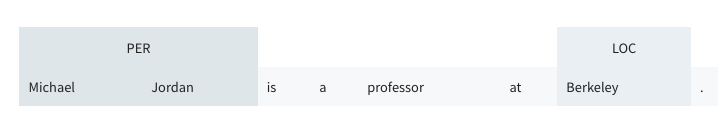
\includegraphics[scale=0.4]{pics/NER.png}
	\caption{Reconocimiento de Entidades Nombradas}
	\label{fig:ner}
\end{figure}


\section{Niveles de descripción lingüística}

El campo de la \textbf{lingüística} aborda el estudio del lenguaje en diferentes niveles de descripción:

\begin{itemize}
  \item \textbf{Fonética y fonología:} estudio de los sonidos del habla.
  \item \textbf{Morfología:} estudio de la estructura de las palabras.
  \item \textbf{Sintaxis:} estudio de la estructura de las oraciones.
  \item \textbf{Semántica:} estudio del significado de las palabras y oraciones.
  \item \textbf{Pragmática:} estudio del uso del lenguaje en el contexto.
\end{itemize}

Estudiemos estos niveles con un poco más de detalle pues conocerlos tiene utilidad a la hora de diseñar sistemas de PLN como se discutirá más adelante.




\subsection{Fonética}

La fonética es la rama de la lingüística que se ocupa del estudio de los sonidos del lenguaje. Examina los órganos utilizados en la producción de sonidos, como la boca, la lengua, la garganta, la nariz, los labios y el paladar. Los sonidos del lenguaje se dividen en vocales y consonantes. Las vocales se producen con poca restricción del flujo de aire desde los pulmones, mientras que las consonantes implican alguna restricción o cierre en el tracto vocal \cite{JohnsonMLSS, fromkin2018introduction}. Además, el Alfabeto Fonético Internacional (AFI) proporciona una notación alfabética para representar los sonidos fonéticos de todos los idiomas.

\subsection{Fonología}

La fonología se centra en el estudio de cómo los sonidos del habla forman patrones y construyen significado. Los fonemas son las unidades básicas de sonido que diferencian el significado de las palabras.
\begin{example}
Por ejemplo, en inglés, la ``p'' y la ``b'' son fonemas distintos porque cambian el significado de las palabras en las que se encuentran (piensen las palabras ``pat'' y ``bat''). 
\end{example}

La fonología también examina las variaciones en la pronunciación de los sonidos en diferentes contextos y dialectos \cite{fromkin2018introduction}.
\subsection{Morfología}

La morfología es el campo de estudio encargado de analizar la estructura interna de las palabras. Los morfemas, que son las unidades mínimas de significado, son los componentes fundamentales de las palabras. 
\begin{example}
Por ejemplo, en la palabra ``deshacer'', los morfemas presentes son ``des-'', ``hacer'' y ``-er''.  
\end{example}

Además, la morfología examina los procesos de formación de palabras, como la derivación, que implica agregar prefijos o sufijos a una palabra existente para crear una nueva palabra con un significado diferente \cite{JohnsonMLSS}.

\begin{example}
Un ejemplo ilustrativo de la morfología derivativa es la palabra en inglés ``revitalization''. En esta palabra, los morfemas ``re+vital+ize+ation'' se combinan para formar una estructura jerárquica en su morfología derivativa, como se muestra en la Figura~\ref{fig:morfo_der}. El sufijo ``ation'' determina la categoría gramatical (part-of-speech) de la palabra derivada, en este caso, un sustantivo (noun). 
\end{example}



\begin{figure}[h]
	\centering
	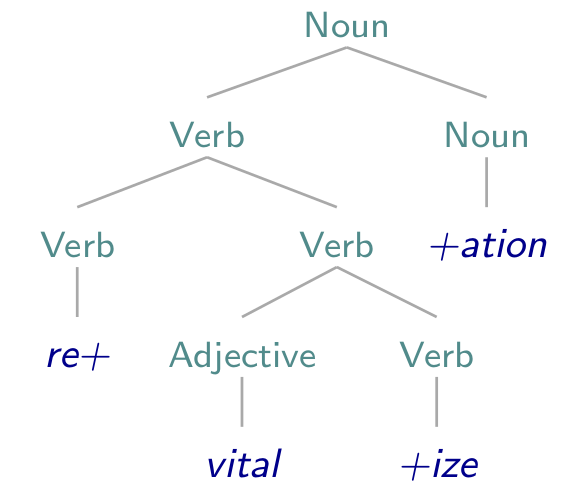
\includegraphics[scale = 0.2]{pics/morphology.png}
	\caption{Árbol Jerárquico de la Morfología Derivativa}
	\label{fig:morfo_der}
\end{figure}

Otra propiedad morfológica importante es la inflexión, que se refiere a los cambios realizados en las palabras para expresar concordancia gramatical, como la conjugación de los verbos o la indicación de género y número en los sustantivos. Por ejemplo, ``el perro'', ``la perra'', ``los perros'', son ejemplos de cómo se aplican las reglas de inflexión en el español para indicar el género y número (singular o plural) en los sustantivos.

\subsection{Sintaxis}

La sintaxis es el estudio de cómo las palabras se combinan para formar frases y oraciones gramaticales. Examina las reglas y estructuras que determinan la organización de las palabras en una oración para un idioma particular y cómo influyen en el significado. La sintaxis también se ocupa de la relación entre las palabras y las funciones que desempeñan dentro de una oración. 
\begin{example}
Por ejemplo, en la oración ``The cat chased the dog'', ``The cat'' es el sujeto, ``chased'' es el verbo y ``the dog'' es el complemento directo \cite{JohnsonMLSS}, tal como muestra el árbol sintáctico en la Figura~\ref{fig:arbol_sintactico}. 
\end{example}

El análisis sintáctico ayuda a identificar \textbf{quién hizo qué a quién} en una oración, lo cual es muy útil para comprender su significado.

\begin{figure}[h]
	\centering
	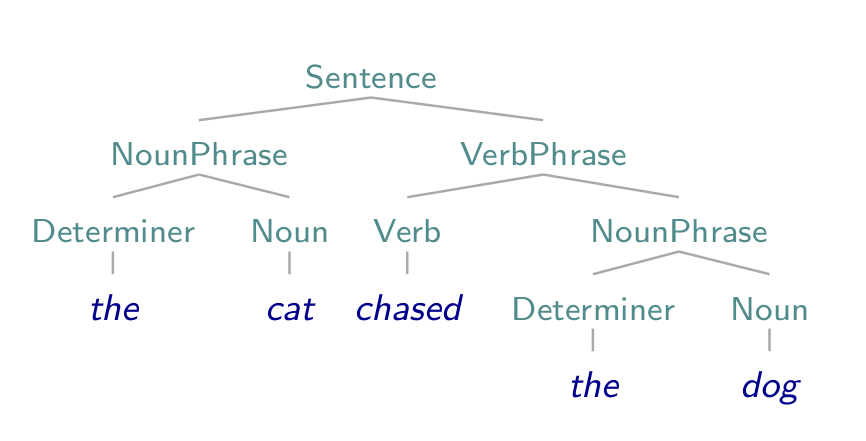
\includegraphics[scale = 0.3]{pics/parseTree1.png}
	\caption{Árbol Sintáctico}
	\label{fig:arbol_sintactico}
\end{figure}




\subsection{Semántica}

La semántica es el estudio del significado de las palabras, frases y oraciones, examinando cómo se construye e interpreta este significado en el contexto del lenguaje. Además, la semántica se interesa por los roles semánticos, que indican la función de cada entidad en una oración.  

\begin{example}
Algunos ejemplos de roles semánticos son: \textcolor[rgb]{0.00,0.00,1.00}{\textbf{agente}} (la entidad que realiza la acción), \textcolor[rgb]{1.00,0.00,0.00}{\textbf{tema}} (la entidad involucrada en la acción) y \textcolor[rgb]{0.00,1.00,0.00}{\textbf{instrumento}} (otra entidad utilizada por el agente para llevar a cabo la acción). En la oración ``El niño cortó la cuerda con un cuchillo'', se puede identificar el agente como \textcolor[rgb]{0.00,0.00,1.00}{\textbf{el niño}}, el tema como \textcolor[rgb]{1.00,0.00,0.00}{\textbf{la cuerda}} y el instrumento como \textcolor[rgb]{0.00,1.00,0.00}{\textbf{un cuchillo}} \cite{JohnsonMLSS}. 
\end{example}



Además de los roles semánticos, la semántica también se ocupa de las relaciones léxicas (o semántica léxica), que son las conexiones entre distintas palabras \cite{yule2016study}.

\begin{example}
Algunos ejemplos de estas relaciones incluyen la sinonimia, que se refiere a palabras con significados similares como ``esconder'' y ``ocultar''; la antonimia, que involucra palabras con significados opuestos como ``alto'' y ``bajo''; y la hiponimia, que establece una relación entre una palabra más específica y otra más general, como ``perro'' y ``animal''. Además, existe la hiperonimia, que representa la relación contraria. 
\end{example}


\subsection{Pragmática}

La pragmática se centra en cómo el contexto influye en la interpretación y el significado de las expresiones lingüísticas. Examina cómo se utilizan las expresiones lingüísticas en situaciones reales y cómo los hablantes interpretan el significado implícito. 

\begin{example}
Por ejemplo, la oración ``Hace frío aquí'' puede interpretarse como una sugerencia implícita parra cerrar las ventanas \cite{fromkin2018introduction}. 
\end{example}


\section{Aprendizaje Automático en PLN}

Dotar a los computadores de habilidades para comprender y producir el lenguaje humano es extremadamente complejo. La tecnología más exitosa actualmente para abordar PLN es el aprendizaje automático supervisado, que consiste en una familia de algoritmos que ``aprenden'' a construir la respuesta del problema en cuestión en base a encontrar patrones en datos de entrenamiento etiquetados. La esencia del aprendizaje automático supervisado es la creación de mecanismos que puedan examinar ejemplos y producir generalizaciones \cite{goldberg2017neural}. Diseñamos un algoritmo cuya entrada es un conjunto de ejemplos etiquetados y cuya salida es una función (o un programa) que recibe una instancia y produce la etiqueta deseada.

Por ejemplo, si la tarea es distinguir entre correos electrónicos de spam y no spam, los ejemplos etiquetados serían correos electrónicos etiquetados como spam y correos electrónicos etiquetados como no spam. Se espera que la función resultante produzca predicciones de etiquetas correctas también para instancias que no ha visto durante el entrenamiento.

\begin{example}
A continuación se muestra un ejemplo etiquetado tanto para la tarea de etiquetado gramatical como la de extracción de entidades nombradas del dataset NER CoNLL-2003\footnote{Fuente: \url{https://www.clips.uantwerpen.be/conll2003/ner/}}. Cada línea contiene un token, una etiqueta de categoría gramatical, una etiqueta de sintagma y una etiqueta de entidad nombrada.

\begin{center}
\begin{verbatim}
U.N.         NNP  I-NP  I-ORG
official     NN   I-NP  O
Ekeus        NNP  I-NP  I-PER
heads        VBZ  I-VP  O
for          IN   I-PP  O
Baghdad      NNP  I-NP  I-LOC
.            .    O     O
\end{verbatim}
\end{center}
\end{example}



A continuación desarrollamos de forma más concreta el uso del aprendizaje automático para tareas de PLN mediante dos ejemplos.

\subsection{Ejemplo 1: Clasificación de Tópicos}

La clasificación de tópicos es una tarea específica de la clasificación de documentos, en la cual se asigna a cada documento una de varias categorías predefinidas, como deportes, política, farándula o economía. La idea fundamental es que las palabras presentes en los documentos pueden ser indicativas del tema que abordan. Sin embargo, crear reglas manuales para esta tarea resulta desafiante debido a la complejidad del lenguaje. La anotación de datos, en la cual personas etiquetan manualmente una colección de documentos según su tema, puede ser de gran ayuda para generar conjuntos de datos de entrenamiento utilizados por algoritmos de aprendizaje automático supervisado. Estos algoritmos aprenden patrones de uso de palabras que facilitan la categorización de los documentos y suelen ser más robustos que las reglas construidas de forma manual.


\subsection{Ejemplo 2: Análisis de Sentimiento}

El análisis de sentimientos se refiere a la aplicación de técnicas PLN para identificar y extraer información subjetiva de conjuntos de datos textuales. Un desafío común en el análisis de sentimientos es la clasificación de la polaridad a nivel de mensaje (MPC), donde las oraciones se clasifican automáticamente en categorías positivas, negativas o neutrales. Las soluciones más avanzadas utilizan modelos de aprendizaje automático supervisado entrenados con ejemplos anotados manualmente.

Una aplicación concreta del análisis de sentimiento es construir un modelo que nos diga si un tweet tiene un sentimiento positivo o negativo respecto a un producto. Para resolver el problema con aprendizaje supervisado primero necesitamos etiquetar manualmente un conjunto de tweets con su sentimiento asociado. Luego debemos entrenar un algoritmo de aprendizaje utilizando estos datos para poder predecir de manera automática el sentimiento asociado a tweets desconocidos. Como podrán imaginar, el etiquetado de datos es una parte fundamental de la solución y puede ser un proceso muy costoso, especialmente cuando se requiere conocimiento especializado para definir la etiqueta.

En este tipo de clasificación, es común transformar las oraciones en vectores de características (cada característica es una columna o dimensión del vector) y aplicar modelos lineales como las Máquinas de Vectores de Soporte (SVM), como se ilustra en la Figura~\ref{fig:senti_class}. Una forma habitual de representar las oraciones o documentos en forma vectorial es mediante el enfoque de la bolsa-de-palabras, donde cada documento se representa como un vector con una columna por cada palabra identificada en el conjunto de documentos (o corpus). Si una palabra está presente en un documento, se asigna un valor distinto de cero en la columna correspondiente, ya sea 1 o la frecuencia de la palabra en el documento. En caso de que la palabra no esté presente, se asigna un valor cero en esa columna.

\begin{figure}[h]
\centering
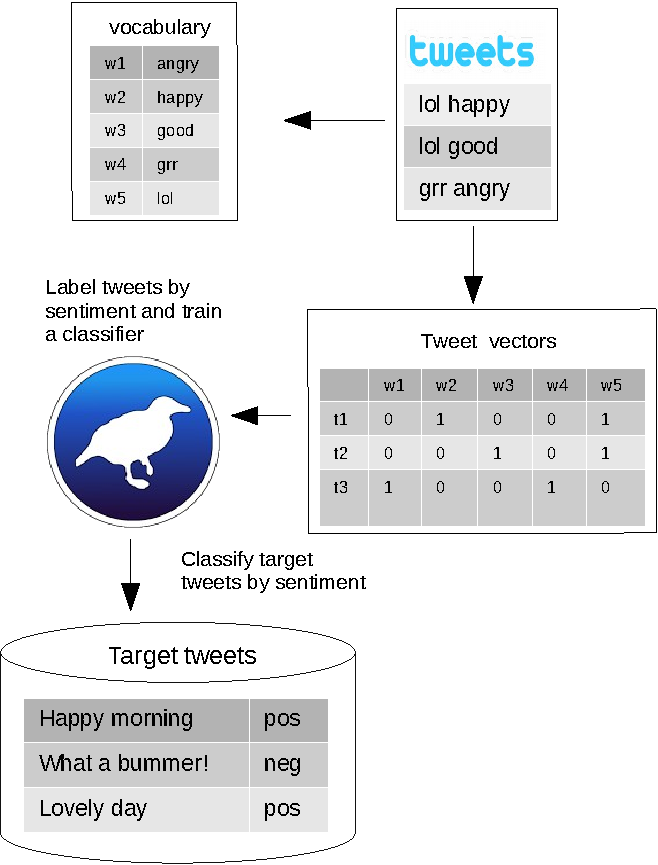
\includegraphics[scale = 0.5]{pics/bagOfwordsClassification.pdf}
\caption{Proceso de Clasificación de Sentimiento en Tweets con Vectores Bolsa-de-Palabras.}
\label{fig:senti_class}
\end{figure}

El objetivo de las SVM es encontrar un hiperplano que separe las representaciones vectoriales de las clases con el margen máximo, logrando la mejor separación entre las clases positivas, negativas y neutrales \cite{jacobbook}, tal como se ilustra en la Figura~\ref{fig:svm}. Una vez encontrado el hiperplano, se puede utilizar para clasificar nuevos tweets en categorías de sentimiento proyectándolos primero en el espacio vectorial de la bolsa-de-palabras y luego determinando en qué lado del hiperplano se encuentra el vector resultante. De esta manera, se asigna una etiqueta de sentimiento (positivo, negativo o neutral) al tweet en base a su posición relativa al hiperplano.

\begin{figure}[h]
\centering
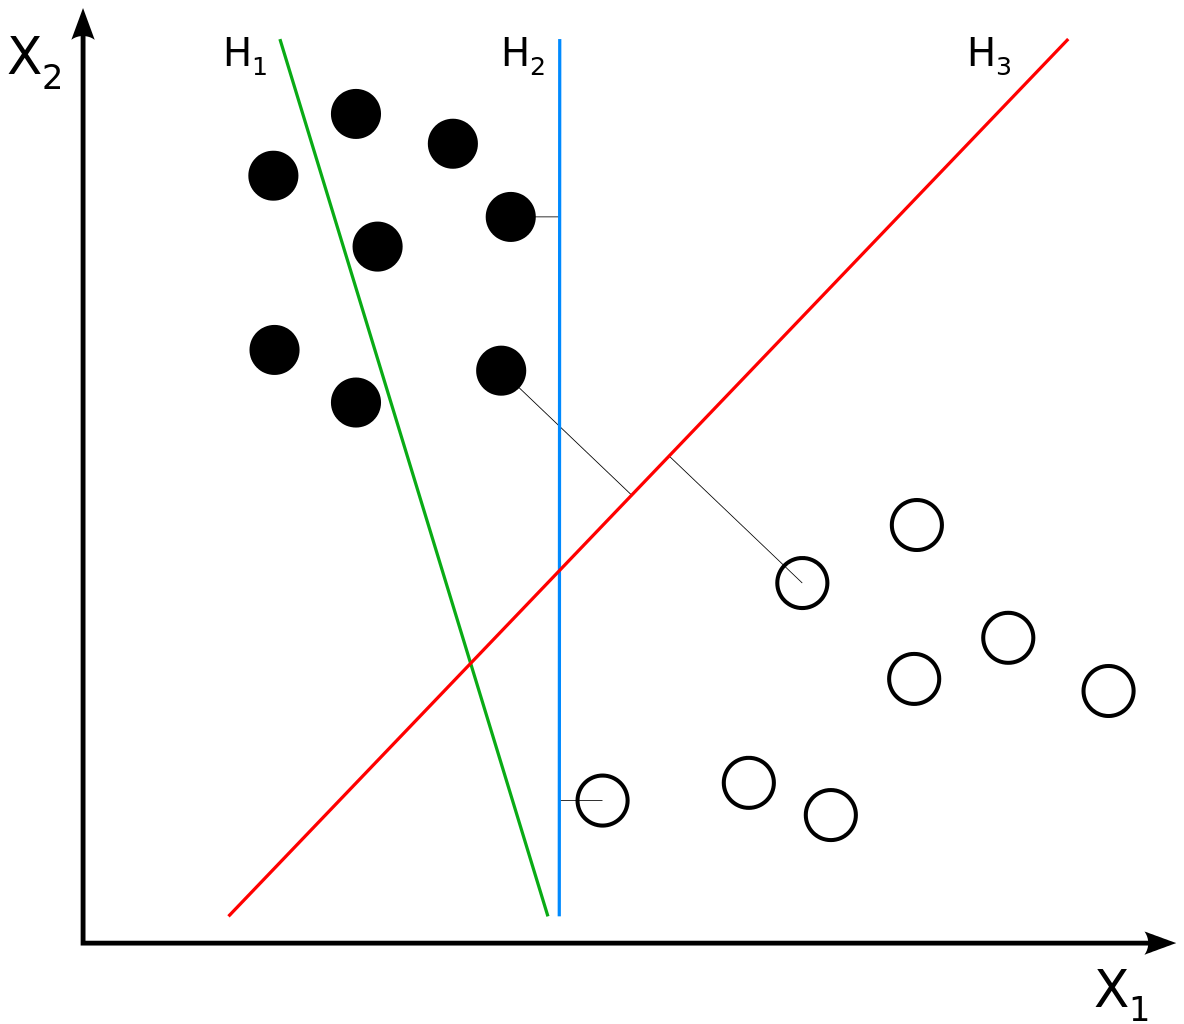
\includegraphics[scale = 0.15]{pics/SVM.png}
\caption{SVM, el hiperplano $H_3$ separa las clases con el margen máximo.}
\label{fig:svm}
\end{figure}





\subsection{Lingüística y Procesamiento del Lenguaje Natural (PNL)}

El conocimiento de las estructuras lingüísticas es fundamental para el diseño de características y el análisis de errores en el Procesamiento del Lenguaje Natural (PNL). Los enfoques de aprendizaje automático en PNL se basan en características que describen y generalizan las instancias de uso del lenguaje. El conocimiento lingüístico orienta la selección y el diseño de estas características, ayudando al algoritmo de aprendizaje automático a encontrar correlaciones entre el uso del lenguaje y las etiquetas objetivo \cite{bender2013linguistic}.

\subsection{Limitaciones del Aprendizaje Supervisado}

Si bien el aprendizaje automático puede resolver satisfactoriamente muchas tareas de Procesamiento del Lenguaje Natural (PLN), no está exento de limitaciones. En primer lugar, la anotación manual de datos requiere recursos humanos y tiempo de trabajo que no están al alcance de todas las organizaciones. Además, los modelos de aprendizaje supervisado pueden tener dificultades para generalizar correctamente a datos que difieren significativamente de los datos de entrenamiento, lo que se conoce como variación de dominio. Para comprender mejor este problema, consideremos las siguientes dos oraciones en el contexto de la clasificación de sentimientos:

\begin{enumerate}
   \item Para mí, la cola era bastante \textcolor[rgb]{0.00,0.00,1.00}{\textbf{pequeña}} y solo tuve que esperar unos 20 minutos, ¡pero valió la pena! :D @raynwise
   \item Extraña espacialidad en Stuttgart. La habitación del hotel es tan \textcolor[rgb]{1.00,0.00,0.00}{\textbf{pequeña}} que apenas puedo moverme, pero los alrededores son inhumanamente vastos y largos bajo construcción.
\end{enumerate}

Podemos observar que la palabra ``pequeña'' tiene una connotación positiva en el contexto de una cola de un banco, pero una connotación negativa en referencia al tamaño de una habitación de hotel. Por lo tanto, un modelo entrenado únicamente con datos de reseñas de hoteles podría tener un mal desempeño al aplicarlo a contextos relacionados con colas de un banco.

Además, los modelos de PLN pueden volverse obsoletos a medida que el uso del lenguaje evoluciona con el tiempo. Por ejemplo, un modelo de clasificación de sentimientos entrenado antes de la aparición de los emojis no tendría en cuenta esta valiosa información. Como resultado, los modelos deben ser monitoreados constantemente y, en muchos casos, reentrenados con nuevos datos para funcionar correctamente en sus entornos de aplicación.

\section{Etiquetado de Datos en PLN}

La construcción de conjuntos de datos de entrenamiento y evaluación para modelos de aprendizaje automático en Procesamiento del Lenguaje Natural (PLN) requiere un enfoque cuidadoso para asegurar que los modelos aprendan a resolver la tarea objetivo de manera efectiva.

En primer lugar, es necesario obtener un corpus (o colección) de documentos objetivo que sean representativos de la tarea en cuestión. A continuación, se debe establecer una guía de anotación para los etiquetadores. Por ejemplo, si la tarea es la clasificación de sentimientos, se recopilan tweets (corpus) y se define una guía que solicita a los anotadores que determinen el sentimiento del autor del tweet en base a tres categorías (positivo, negativo, neutral).

Luego, se reclutan anotadores que deben ser independientes y tener suficientes conocimientos en el lenguaje y la tarea para realizar etiquetados consistentes. Esto suele llevarse a cabo a través de plataformas en línea especializadas.

Los anotadores etiquetan los documentos de manera sistemática y suelen ser evaluados de forma continua. Para evaluar su desempeño, se suelen pre-etiquetar algunos ejemplos con el fin de determinar si los anotadores comprenden correctamente el objetivo de la anotación.

A continuación, se comparan las anotaciones de los distintos etiquetadores utilizando criterios de concordancia inter-anotador (inter-annotator agreement). Para problemas de clasificación, dos métricas comunes son el coeficiente Kappa de Cohen y el coeficiente Kappa de Fleiss.

El coeficiente Kappa de Cohen se calcula utilizando la siguiente fórmula:

\[
K = \frac{P_o - P_e}{1 - P_e}
\]

donde \(P_o\) es la proporción observada de acuerdo entre los anotadores y \(P_e\) es la proporción esperada de acuerdo por azar. El coeficiente Kappa de Cohen mide la proporción de acuerdo entre los anotadores que es superior al acuerdo esperado al azar. Un valor de \(K\) cercano a 1 indica un buen acuerdo entre los anotadores, mientras que un valor cercano a 0 indica un acuerdo similar al que se podría esperar al azar.

El coeficiente Kappa de Fleiss también se utiliza para medir la concordancia inter-anotador en problemas de clasificación con múltiples anotadores. A diferencia del coeficiente Kappa de Cohen, el coeficiente Kappa de Fleiss tiene en cuenta el acuerdo más allá de dos anotadores y se calcula de la siguiente manera:

\[
K = \frac{\overline{P_o} - \overline{P_e}}{1 - \overline{P_e}}
\]

donde \(\overline{P_o}\) es la proporción media observada de acuerdo entre los anotadores y \(\overline{P_e}\) es la proporción media esperada de acuerdo por azar.

Finalmente, se lleva a cabo un proceso de consolidación de las anotaciones. Por ejemplo, si se cuenta con tres anotadores, se puede utilizar una regla de mayoría simple para asignar las etiquetas finales a los datos. En algunos casos, los ejemplos en los que hay desacuerdo pueden ser etiquetados nuevamente por anotadores más experimentados, mientras que en otros casos se eliminan del conjunto de datos. Todas estas decisiones pueden tener consecuencias en la calidad de los conjuntos de datos y, en consecuencia, en el rendimiento de los modelos entrenados con estos datos.

Al conjunto de datos resultante del proceso de consolidación se le llama ``gold standard'' o ``ground truth'' y se utiliza posteriormente para entrenar modelos de aprendizaje automático. 

Referencias recomendadas en anotación de datos para PLN se encuentran en los libros~\cite{fort2016collaborative} y~\cite{pustejovsky2012natural}.


\subsection{Supervisión a Distancia}

En algunos casos, es posible etiquetar datos de manera semi-automática con una técnica llamada supervisón a distancia, lo que permite ahorrar costos de anotación. Un ejemplo de esto es el enfoque de anotación de emoticones utilizado en la clasificación de sentimientos en tweets. En este enfoque, se utiliza la API de Twitter para recopilar tweets que contengan emoticones positivos \textcolor[rgb]{0.00,0.00,1.00}{\textbf{:)}} o negativos \textcolor[rgb]{1.00,0.00,0.00}{\textbf{:(}}, y luego se etiquetan los tweets según la polaridad indicada por el emoticón~\cite{Read2005}. El emoticón se \textbf{elimina} del contenido del tweet. Este enfoque también se ha ampliado utilizando hashtags como \#rabia y emojis. Sin embargo, no es trivial encontrar técnicas de supervisión a distancia que sean aplicables a todos los tipos de problemas en PLN.

\subsection{Crowdsourcing}
Las plataformas de crowdsourcing, como \textbf{Amazon Mechanical Turk (AMT)}\footnote{\url{https://www.mturk.com/}}, ofrecen la posibilidad de etiquetar datos a gran escala mediante el pago a etiquetadores remotos. Si bien este enfoque permite la anotación masiva de datos, es difícil garantizar la calidad esperada por parte de los anotadores. Sin embargo, ha sido gracias a este enfoque que se ha logrado la proliferación de numerosos conjuntos de datos para entrenar modelos supervisados en PLN. En \cite{snow2008cheap} se realiza una comparación exhaustiva sobre la calidad de las anotaciones obtenidas con AMT para diversas tareas de PLN.  Los resultados muestran que las anotaciones obtenidas son comparables a las de los anotadores expertos. 

\section{Paradigmas de Aprendizaje Automático}

Hasta el año 2010, el Procesamiento del Lenguaje Natural (PLN) se basaba en modelos de aprendizaje poco profundos y en características manuales. Por ejemplo, en 2013, el taller de Evaluación Semántica (SemEval) organizó la tarea de "Análisis de sentimientos en Twitter" \cite{Semeval2013}. Esta tarea se dividió en dos sub-tareas: el nivel de expresión y el nivel del mensaje. El nivel de expresión se centró en determinar la polaridad del sentimiento de un mensaje según una entidad marcada dentro de su contenido, mientras que el nivel del mensaje buscaba determinar la polaridad según el mensaje en general. Los organizadores proporcionaron conjuntos de datos de entrenamiento y prueba para ambas tareas \cite{Semeval2013}.

El equipo que logró el mejor rendimiento en ambas tareas, entre 44 equipos participantes, fue el equipo llamado \emph{NRC-Canada} \cite{Mohammad2013}. Este equipo propuso un enfoque supervisado utilizando un clasificador SVM lineal y características hechas a mano para representar los tweets. Algunas de estas características fueron:

\begin{enumerate}
  \item N-gramas de palabras (similares a los vectores bolsa-de-palabras, pero con secuencias contiguas de $n$ palabras).
  \item N-gramas de caracteres (similar a lo anterior, pero con secuencias contiguas de $n$ caracteres).
  \item Etiquetas de categorías gramaticales.
  \item Clusters de palabras entrenadas con el método de Brown \cite{brown1992class}.
  \item El número de palabras alargadas (palabras con un carácter repetido más de dos veces).
  \item El número de palabras con todas las letras en mayúscula.
  \item La presencia de emoticones positivos o negativos.
  \item El número de negaciones individuales.
  \item El número de secuencias contiguas de puntos, signos de interrogación y signos de exclamación.
  \item Características derivadas de lexicones de polaridad \cite{Mohammad2013} (listas de palabras con sentimiento asociado). Dos de estos lexicones se generaron utilizando el método PMI (point-wise mutual information) a partir de tweets anotados con hashtags y emoticones.
\end{enumerate}

Cabe destacar que todas estas características se concatenan para crear un único vector por cada tweet, generando una representación de alta dimensión.

Hasta el año 2014, la mayoría de los sistemas del estado-del-arte en PLN se basaban en el paradigma de ingeniería de características (diseño manual de vectores de características) junto con modelos de aprendizaje automático superficiales, como SVM y CRF. Diseñar las características de un sistema de PLN ganador requería un amplio conocimiento específico del dominio. El sistema desarrollado por el equipo NRC-Canada se construyó antes de que el aprendizaje profundo (o deep learning) se volviera popular en el campo del PLN. 

Por otro lado, los sistemas de aprendizaje profundo han revolucionado el campo del PLN. Estos sistemas se basan en redes neuronales profundas para aprender automáticamente buenas representaciones utilizando técnicas como los vectores de palabras (word embeddings) y arquitecturas especializadas como las redes neuronales recurrentes y los Transformers. Estos modelos requieren grandes volúmenes de datos y un alto poder computacional para su entrenamiento efectivo. Las grandes cantidades de datos textuales disponibles en los últimos años, junto con los procesadores de la tarjeta gráfica de múltiples núcleos (GPU y TPU) más rápidos, han sido fundamentales para el éxito del aprendizaje profundo en PLN.

\begin{figure}[h]
	\centering
	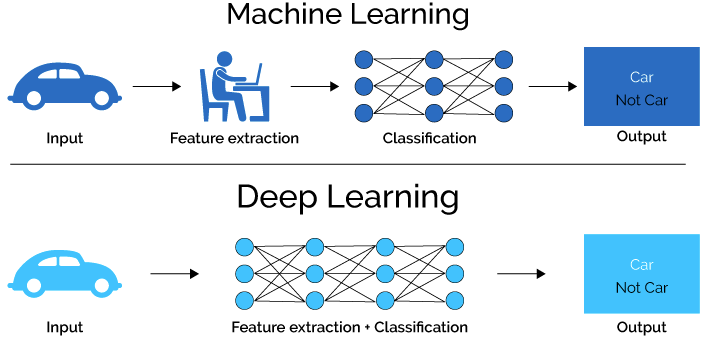
\includegraphics[scale=0.25]{pics/MLvsDL.png}
	\caption{Ingeniería de Características vs Aprendizaje Profundo}
	\label{fig:MLvsDL}
\end{figure}

\paragraph{Aprendizaje Profundo y Conceptos Lingüísticos}
Si los modelos de aprendizaje profundo pueden aprender representaciones automáticamente, ¿siguen siendo útiles los conceptos lingüísticos (por ejemplo, sintaxis, morfología)? Algunos defensores del aprendizaje profundo argumentan que estas propiedades lingüísticas inferidas y diseñadas manualmente no son necesarias, y que la red neuronal aprenderá estas representaciones intermedias (o equivalentes o mejores) por sí misma \cite{goldberg2016primer}. Aún no hay un consenso definitivo al respecto. Goldberg cree que muchos de estos conceptos lingüísticos pueden ser inferidos por la red por sí misma si se le proporciona suficiente cantidad de datos. Sin embargo, en muchos otros casos no disponemos de suficientes datos de entrenamiento para la tarea que nos interesa, y en estos casos proporcionar a la red los conceptos generales más explícitos puede ser muy valioso.


\section{Historia de PLN}

Los orígenes de PLN se remontan a los años 50 con el famoso test de Alan Turing: una máquina será considerada inteligente cuando sea capaz de conversar con una persona sin que esta pueda determinar si está hablando con una máquina o un ser humano. A lo largo de su historia, la disciplina ha experimentado tres grandes períodos: el racionalismo, el empirismo y el aprendizaje profundo \cite{deng2018deep}.

El período del racionalismo abarcó desde 1950 hasta 1990, donde las soluciones consistían en diseñar reglas manuales para incorporar mecanismos de conocimiento y razonamiento. Un ejemplo emblemático de esta época es ELIZA, un agente de conversación (o chatbot) desarrollado por Joseph Weizenbaum, que simulaba ser un psicoterapeuta rogeriano. También se destaca en esa época el sistema MARGIE, utilizado para estructurar información del mundo real en ontologías de conceptos.

A partir de la década de los 90, el enfoque de PLN se inclinó hacia el empirismo, con el diseño de métodos estadísticos y de aprendizaje automático construidos sobre corpus de datos etiquetados. En este período, las reglas ya no se construían manualmente, sino que se ``aprendían'' a partir de los datos. Algunos modelos representativos de esta época son los filtros de spam basados en modelos Bayesianos, las cadenas de Markov ocultas para la extracción de categorías sintácticas y los modelos probabilísticos de IBM para la traducción automática. Estos modelos se caracterizaban por ser poco profundos en su estructura de parámetros y dependían de características manualmente diseñadas para representar la entrada.

A partir del año 2010, las redes neuronales artificiales, que son una familia de modelos de aprendizaje automático, comenzaron a mostrar resultados sobresalientes en varias tareas emblemáticas de PLN \cite{collobert2011natural}. Estos modelos utilizan una jerarquía de parámetros (o capas) para representar la entrada (texto) y encontrar representaciones adecuadas para la tarea en cuestión, en lo que se conoce como ``aprendizaje profundo''. Se caracterizan por tener muchos más parámetros que los modelos anteriores, superando la barrera del millón en algunos casos, y requieren grandes volúmenes de datos para su entrenamiento. Estos modelos pueden ser pre-entrenados con texto no etiquetado, como libros, Wikipedia, textos de redes sociales y de la web, para encontrar representaciones iniciales de palabras y oraciones (conocidas como word embeddings), que luego pueden ser adaptadas para la tarea específica utilizando datos etiquetados (proceso conocido como fine-tuning). Entre estos modelos se destacan Word2Vec \cite{Mikolov2013}, BERT \cite{kenton2019bert}, GPT-3 \cite{brown2020language} y otros grandes modelos de lenguaje que han surgido recientemente (ChatGPT, Google Bard).

Estos modelos han ido perfeccionándose en los últimos años, logrando resultados cada vez mejores en casi todos los problemas del área. Sin embargo, este progreso no ha estado exento de controversias. El aumento exponencial en la cantidad de parámetros de cada nuevo modelo en comparación con su predecesor ha hecho que la construcción de estos modelos requiera recursos computacionales y energéticos que solo están al alcance de unos pocos. Además, varios estudios han demostrado que estos modelos aprenden y reproducen sesgos y prejuicios presentes en los textos utilizados para su entrenamiento, como los relacionados con género, religión y raza. Un ejemplo destacado es el despido de la investigadora Timmnit Gebru de Google, luego de que se le negara el permiso para publicar un artículo que revelaba estos problemas \cite{bender2021dangers}.



\section{Conclusiones y Estructura del Apunte}
En este capítulo, hemos explorado el desafío de comprender y generar lenguaje utilizando la computación. El aprendizaje automático supervisado se ha destacado como una de las principales técnicas utilizadas para abordar este desafío. También discutimos las limitaciones y desafíos que enfrenta el Procesamiento del Lenguaje Natural (PLN), como la anotación de datos, la generalización a nuevos dominios y la evolución del lenguaje, entre otros aspectos que requieren atención. Finalmente, hemos visto cómo el aprendizaje profundo ha demostrado mejoras significativas en el rendimiento de los modelos de PLN. Estos modelos basados en redes neuronales han logrado superar barreras anteriores al ser capaces de capturar patrones más complejos y aprender representaciones más ricas del lenguaje.

El resto de este apunte se estructura de la siguiente manera: en el Capítulo~\ref{cap_ir} se presenta el modelo de espacio vectorial junto a la discplina hermana de PLN: la recuperación de información. En el Capítulo~\ref{cap_plm} se discuten los modelos de lenguaje probabilísticos basados en n-gramas. En el Capítulo~\ref{cap_nb}, formalizamos la tarea de clasificación de texto e introducimos el modelo naïve bayes. Luego, en el Capítulo~\ref{cap_lineales}, se presentan los modelos lineales en PLN, y en el Capítulo~\ref{cap_redes}, se introducen las redes neuronales. Los vectores de palabras o ``word embeddings'' se discuten en el Capítulo~\ref{cap_embeddings}. Las tareas de etiquetado de secuencia, como el etiquetado gramatical y la extracción de entidades nombradas, se formalizan en el Capítulo~\ref{cap_etisec}, junto con modelos clásicos para esta tarea, como las cadenas de Markov ocultas y los Conditional Random Fields.

A partir del Capítulo~\ref{cap_cnn}, se discuten arquitecturas especializadas de redes neuronales para PLN. Las redes convolucionales se tratan en el Capítulo~\ref{cap_cnn}, las recurrentes en el Capítulo~\ref{cap_rnn}, los modelos secuencia a secuencia, junto con los modelos de atención, en el Capítulo~\ref{cap_sec}, y finalmente, la arquitectura de Transformer se desarrolla en el Capítulo~\ref{cap_trans}.

Cerramos el apunte en el Capítulo~\ref{cap_llm}, donde se presentan modelos modernos de vectores de palabras contextualizados y los grandes modelos de lenguaje.
